\documentclass[10pt,conference,a4paper]{IEEEtran}
\IEEEoverridecommandlockouts

\usepackage[utf8]{inputenc}
\usepackage[T1]{fontenc}
\usepackage[brazil]{babel}
\usepackage{amsmath,amssymb}
\usepackage{array}
\usepackage{balance}
\usepackage{booktabs}
\usepackage{cite}
\usepackage{graphicx}
\usepackage{microtype}
\usepackage{tikz}
\usepackage{url}
\usetikzlibrary{arrows.meta,fit,positioning}

\graphicspath{{../figuras/}}
\emergencystretch=2em
\renewcommand{\abstractname}{Resumo}
\renewcommand{\IEEEkeywordsname}{Palavras-chave}
\newcounter{algoritmo}

\title{Avaliação do DeepNPTS e de Modelos de Referência para Previsão
Mensal de Irradiância Global Horizontal em Localidades de Fábricas de
Veículos Elétricos}

\author{Gustavo de Melo Nascimento, Thales Wulfert Cabral e Gustavo Fraidenraich%
\thanks{Os autores são da Faculdade de Engenharia Elétrica e de Computação,
Universidade Estadual de Campinas, Campinas, SP, Brasil. E-mails:
g239679@dac.unicamp.br, t264377@dac.unicamp.br e gfraiden@unicamp.br.}}

\begin{document}

\maketitle

\begin{abstract}
Este artigo avalia o Deep Non-Parametric Time Series Forecaster (DeepNPTS) na
previsão mensal de Irradiância Global Horizontal (GHI), com horizonte de um
mês, em dez localidades. Dados da National Solar Radiation Database de
2019--2024 são agregados por mês, normalizados e quantizados com parâmetros
pré-teste. O DeepNPTS discreto do GluonTS é comparado a três referências
simples e seis modelos aprendidos. O protocolo retrospectivo utiliza 48 alvos
de treinamento, 12 origens \textit{walk-forward} de teste por localidade,
cinco sementes e parâmetros fixos durante o teste. A climatologia obteve o
menor macro-MAE, 12,07 W/m$^2$; o DeepNPTS obteve 17,70 W/m$^2$, ficou em 9º
lugar entre 10 métodos e superou apenas a persistência. Em relação ao DeepAR,
o DeepNPTS teve maior CRPS e intervalos 4,10 vezes mais largos, embora sua
cobertura tenha ficado mais próxima do nível nominal de 90\%. Os resultados
se restringem à janela retrospectiva estudada.
\end{abstract}

\begin{IEEEkeywords}
Irradiância solar, GHI, previsão probabilística, séries temporais, DeepNPTS.
\end{IEEEkeywords}

\section{Introdução}
\label{sec:introducao}

A disponibilidade do recurso solar condiciona a produção fotovoltaica e
influencia decisões de dimensionamento, planejamento e operação energética.
Previsões de irradiância podem reduzir a incerteza associada a essas decisões,
mas sua
formulação depende do horizonte, da resolução e das informações meteorológicas
disponíveis \cite{antonanzas2016,voyant2017,yang2018}.

Este trabalho considera a Irradiância Global Horizontal (GHI), a irradiância
total incidente em uma superfície horizontal. Em termos das componentes direta
e difusa,

\begin{equation}
  \mathrm{GHI}=\mathrm{DHI}+\mathrm{DNI}\cos(\theta_z),
  \label{eq:ghi}
\end{equation}

\noindent em que DHI é a irradiância difusa horizontal, DNI é a irradiância
direta normal e $\theta_z$ é o ângulo zenital solar \cite{duffie2013}. A GHI é
empregada por representar, em W/m$^2$, a disponibilidade solar sobre o plano
horizontal e por integrar produtos padronizados da National Solar Radiation
Database (NSRDB) \cite{sengupta2018}. A variável-alvo deste estudo é a média
mensal de GHI, não energia nem produção fotovoltaica.

A previsão de uma série mensal com horizonte de um mês pode apoiar comparações
de localidades e análises preliminares de planejamento. A agregação mensal
atenua flutuações intradiárias e evidencia a sazonalidade, mas fornece apenas
doze observações por ano \cite{antonanzas2016,voyant2022}. Nesse regime,
modelos flexíveis devem ser confrontados com referências sazonais simples.

A literatura de previsão solar abrange métodos estatísticos, aprendizado de
máquina e redes neurais \cite{voyant2017,sobri2018}. Neste estudo, XGBoost
\cite{chen2016}, Perceptron Multicamadas (MLP) \cite{hornik1989}, Rede Neural
Recorrente (RNN) \cite{elman1990}, Long Short-Term Memory (LSTM)
\cite{hochreiter1997} e DilatedRNN \cite{chang2017} são os modelos aprendidos
pontuais. Persistência, sazonal ingênuo e climatologia mensal são as
referências simples.

Modelos globais compartilham parâmetros entre séries relacionadas. O DeepAR
aprende uma distribuição preditiva por meio de uma rede autorregressiva global
\cite{salinas2020}. O DeepNPTS também explora séries relacionadas, mas sua
variante discreta aprende probabilidades sobre os valores do contexto, sem
fixar uma família paramétrica para a distribuição preditiva
\cite{rangapuram2023}. Essa característica motiva sua avaliação neste conjunto
de séries curtas, mas não garante maior acurácia em qualquer aplicação.

O objetivo é verificar se o DeepNPTS discreto de \cite{rangapuram2023},
implementado no GluonTS, biblioteca descrita em \cite{alexandrov2020}, supera
referências sazonais e modelos aprendidos na previsão da GHI média do mês
seguinte. Todos usam os mesmos alvos e origens temporais, embora as entradas
respeitem cada arquitetura, como detalhado na Seção~\ref{sec:metodo}. As
fábricas definem somente os pontos geográficos; não são usados dados de carga,
geração ou operação industrial.

\subsection{Principais contribuições}

As contribuições são: (i) avaliação do DeepNPTS discreto como modelo
global das dez séries relacionadas; (ii) comparação com três referências
simples e seis modelos aprendidos sob as mesmas origens temporais; (iii)
protocolo auditável com transformações pré-teste, cinco sementes e métricas
pontuais e probabilísticas; e (iv) interpretação descritiva das limitações de
uma janela retrospectiva curta, sem alegação de pioneirismo ou superioridade
universal.

O restante do artigo está organizado da seguinte forma. A Seção~II descreve o
sistema e o protocolo; a Seção~III apresenta a configuração e as métricas; a
Seção~IV discute os resultados; e a Seção~V reúne as conclusões.

\begin{figure*}[!t]
\centering
\resizebox{0.98\textwidth}{!}{%
\begin{tikzpicture}[
  grupo/.style={draw,dashed,rounded corners=1pt,minimum height=3.1cm,inner sep=4pt},
  caixa/.style={draw,align=center,minimum height=0.72cm,font=\scriptsize,fill=white},
  titulo/.style={align=center,font=\scriptsize\bfseries},
  rotulo/.style={font=\scriptsize},
  seta/.style={-{Latex[length=2mm]},thick}
]
\node[grupo,minimum width=2.45cm] (ga) at (0,0) {};
\node[titulo] at ([yshift=-0.32cm]ga.north) {Séries relacionadas};
\node[caixa,minimum width=1.85cm] (dados) at ([yshift=-1.55cm]ga.north)
  {GHI diária\\NSRDB\\2019--2024};
\node[rotulo] at ([yshift=-0.25cm]ga.south) {(a)};

\node[grupo,minimum width=2.65cm] (gb) at (2.95,0) {};
\node[titulo] at ([yshift=-0.32cm]gb.north) {Auditoria e agregação};
\node[caixa,minimum width=2.05cm] (audit) at ([yshift=-1.15cm]gb.north)
  {Cobertura, lacunas,\\duplicidades e sinais};
\node[caixa,minimum width=2.05cm,below=0.22cm of audit] (mensal)
  {Média mensal};
\draw[seta] (audit)--(mensal);
\node[rotulo] at ([yshift=-0.25cm]gb.south) {(b)};

\node[grupo,minimum width=3.05cm] (gc) at (6.15,0) {};
\node[titulo] at ([yshift=-0.32cm]gc.north) {Transformação e entradas};
\node[caixa,minimum width=2.35cm] (transforma) at ([yshift=-1.15cm]gc.north)
  {Min--max pré-teste,\\saturação e quantização};
\node[caixa,minimum width=2.35cm,below=0.22cm of transforma] (janelas)
  {Janelas, atributos\\e localidade};
\draw[seta] (transforma)--(janelas);
\node[rotulo] at ([yshift=-0.25cm]gc.south) {(c)};

\node[grupo,minimum width=3.55cm] (gd) at (10.05,0) {};
\node[titulo] at ([yshift=-0.32cm]gd.north) {Modelos globais e referências};
\node[caixa,minimum width=2.85cm] (aprendidos) at ([yshift=-1.15cm]gd.north)
  {XGBoost, MLP, RNN, LSTM,\\DilatedRNN, DeepAR e DeepNPTS};
\node[caixa,minimum width=2.85cm,below=0.22cm of aprendidos] (baselines)
  {Persistência, sazonal\\e climatologia};
\node[rotulo] at ([yshift=-0.25cm]gd.south) {(d)};

\node[grupo,minimum width=2.85cm] (ge) at (13.85,0) {};
\node[titulo] at ([yshift=-0.32cm]ge.north) {Teste retrospectivo};
\node[caixa,minimum width=2.25cm] (origens) at ([yshift=-1.15cm]ge.north)
  {Um passo sem\\reajuste};
\node[caixa,minimum width=2.25cm,below=0.22cm of origens] (amostras)
  {Ponto, amostras\\e intervalos};
\draw[seta] (origens)--(amostras);
\node[rotulo] at ([yshift=-0.25cm]ge.south) {(e)};

\node[grupo,minimum width=2.65cm] (gf) at (17.05,0) {};
\node[titulo] at ([yshift=-0.32cm]gf.north) {Avaliação};
\node[caixa,minimum width=2.05cm] (metrica) at ([yshift=-1.15cm]gf.north)
  {Métricas locais\\e macro-MAE};
\node[caixa,minimum width=2.05cm,below=0.22cm of metrica] (incerteza)
  {Incerteza\\probabilística};
\draw[seta] (metrica)--(incerteza);
\node[rotulo] at ([yshift=-0.25cm]gf.south) {(f)};

\draw[seta] (dados.east)--(audit.west);
\draw[seta] (mensal.east)--(transforma.west);
\draw[seta] (janelas.east)--(aprendidos.west);
\draw[seta] (aprendidos.east)--(origens.west);
\draw[seta] (amostras.east)--(metrica.west);
\end{tikzpicture}%
}
\caption{Fluxo do sistema: séries relacionadas, auditoria e agregação,
transformação e representações específicas de cada arquitetura, ajuste global,
teste retrospectivo e avaliação.}
\label{fig:sistema}
\end{figure*}

\section{Sistema e método experimental}
\label{sec:metodo}

A Fig.~\ref{fig:sistema} resume o fluxo, cujos blocos são descritos na mesma
ordem.



\noindent\textbf{Estágio (a) -- dados.} Cada localidade $\ell\in\mathcal L$
fornece uma série diária $S_\ell$. As dez séries possuem a mesma variável e
frequência, mas escalas e sazonalidades locais distintas.

\noindent\textbf{Estágio (b) -- auditoria e agregação.} O sistema verifica
datas, duplicidades, lacunas, valores não finitos e GHI negativa e calcula a
média de cada mês civil. Os arquivos preservados contêm médias diárias
derivadas de consultas com intervalo de 60 minutos; as respostas horárias
brutas não foram preservadas e não podem ser reconstituídas a partir dessas
médias.

\noindent\textbf{Estágio (c) -- transformação e representações.} Para cada
localidade, os limites min--max são estimados sem alvos do teste. Valores fora
desses limites são saturados em $[0,1]$ e quantizados uniformemente. Essa
discretização é uma escolha experimental do pipeline, não um requisito do
DeepNPTS. Modelos tabulares recebem 12 defasagens, médias móveis, calendário e
codificação da localidade; redes recorrentes recebem a sequência cronológica e
covariáveis separadas, concatenadas à representação temporal antes da camada
densa; DeepNPTS e DeepAR recebem as séries transformadas e a categoria estática.
Assim, alvos e origens são comuns, mas as entradas respeitam cada arquitetura.

\noindent\textbf{Estágio (d) -- ajuste.} Para cada modelo aprendido e semente,
há um único modelo final global, compartilhado pelas dez localidades; não é
ajustado um modelo por fábrica. Quando aplicável, a complexidade é escolhida em
uma validação cronológica e o modelo é reinicializado e reajustado em todo o
período pré-teste. As referências simples não têm ajuste conjunto.

\noindent\textbf{Estágio (e) -- teste.} Em cada origem, o histórico inclui
somente meses já disponíveis e o mês seguinte é previsto. O valor de
referência de um mês de 2024 integra o contexto da origem seguinte,
mas os parâmetros permanecem fixos. Portanto, o protocolo não prevê os doze
meses conjuntamente em dezembro de 2023.

\noindent\textbf{Estágio (f) -- escala física e avaliação.} As saídas são
invertidas para W/m$^2$. Na inversão aplica-se apenas o piso físico de zero,
sem corte superior no máximo do treinamento; logo, erros e caudas acima desse
máximo permanecem representados nos modelos capazes de extrapolar. O DeepNPTS
discreto, por construção, amostra somente valores de seu contexto. Calculam-se
métricas por localidade e médias não ponderadas entre as dez localidades.

\subsection{DeepNPTS e consolidação de sementes}

No DeepNPTS discreto, $t$ denota o último mês observado e
$\mathbf z_{\ell,t}$ reúne os $C$ valores transformados do contexto da
localidade $\ell$. Uma rede global combina esse contexto, atributos de tempo e
o \textit{embedding} da localidade para definir probabilidades
$p_{\ell,t,j}$ sobre suas posições. A função de distribuição acumulada (CDF)
preditiva de um passo é

\begin{equation}
 \widehat F_{\ell,t+1}(x)=\sum_{j=1}^{C}p_{\ell,t,j}
 \mathbb I(z_{\ell,t-C+j}\le x),\qquad \sum_{j=1}^{C}p_{\ell,t,j}=1.
 \label{eq:deepnpts}
\end{equation}

\noindent em que $x$ é um valor de comparação e $\mathbb I$ vale 1 quando a condição é
verdadeira e 0 caso contrário. Equivalentemente, sorteia-se a posição
$J\sim\mathrm{Categorical}(p_{\ell,t,1:C})$ e
$\widetilde z_{\ell,t+1}=z_{\ell,t-C+J}$. A repetição produz amostras e
quantis. Trata-se do estimador discreto do GluonTS 0.16.2, com correção local
restrita ao registro dos embeddings categóricos no PyTorch. Portanto, o modelo
avaliado é o estimador neural não paramétrico, e não um suavizador
determinístico por similaridade e recência.

O treinamento minimiza o escore de probabilidade ranqueado (RPS) normalizado
implementado pela distribuição discreta do GluonTS, conforme a formulação
não paramétrica do modelo \cite{rangapuram2023}.

As previsões dos modelos pontuais aprendidos são consolidadas pela média das
cinco execuções em cada origem. As referências simples produzem uma única
previsão por origem.
Para DeepNPTS e DeepAR, as amostras das cinco sementes são reunidas em uma
única mistura empírica; a mediana dessa mistura é a previsão pontual, e seus
quantis definem os intervalos. Denotando por $\mathcal S$ o conjunto de
sementes e por $B_s$ o número de amostras por semente, cada distribuição final
contém $B=B_s|\mathcal S|$ valores, sem primeiro reduzir cada semente a um
único ponto.

\subsection{Algoritmo compacto}

\refstepcounter{algoritmo}\label{alg:sistema}
\noindent\textbf{Algoritmo \thealgoritmo: Treinamento global e avaliação}

\noindent\fbox{%
\begin{minipage}{0.94\columnwidth}
\scriptsize
\textbf{Entrada:} séries $\mathcal D$, modelos $\mathcal M$, sementes
$\mathcal S$, contexto $C$, horizonte $h$, corte $c$, níveis $Q$ e origens
$\mathcal O$.\par
\textbf{1:} auditar e agregar cada série por mês civil.\par
\textbf{2:} ajustar a transformação antes de $c$ e construir, para cada
arquitetura, entradas causais de contexto $C$ e horizonte $h$.\par
\textbf{3:} para cada $m\in\mathcal M$ e $s\in\mathcal S$, selecionar a
complexidade, quando aplicável, sem usar o teste e ajustar um modelo final
global no pré-teste.\par
\textbf{4:} em cada $o\in\mathcal O$, truncar o histórico, prever sem reajuste
e inverter a escala com piso zero.\par
\textbf{5:} consolidar sementes, calcular métricas locais e médias macro e
ordenar descritivamente os métodos pelo macro-MAE.\par
\textbf{Saída:} previsões, amostras, intervalos, métricas e ranking.
\end{minipage}}

\section{Configuração experimental e métricas}
\label{sec:configuracao}

Foram utilizados dados do produto GOES Aggregated PSM v4 da NSRDB
\cite{sengupta2018,nlr2026}. A NSRDB combina informação de satélite e modelos
físicos; seus valores são referência modelada, não medição de solo. A consulta
original adotou intervalo de 60 minutos, e o projeto preserva médias das 24
horas de cada dia, posteriormente agregadas por mês civil.

As localidades são BYD Camaçari, BMW San Luis Potosí, Ford Rouge, GM Factory
Zero, Hyundai Georgia, Lucid Casa Grande, Rivian Normal e Tesla Fremont, Nevada
e Texas. Cada série possui 72 meses de 2019 a 2024. Com contexto de 12 meses,
os 60 alvos elegíveis cobrem 2020--2024: os 48 primeiros (80\%) formam o
treinamento (2020--2023), e os 12 últimos (20\%), o teste (2024). O ano de 2019
fornece o primeiro contexto. A divisão é cronológica. A janela de 2024 já foi
inspecionada durante o desenvolvimento; a análise é retrospectiva e
exploratória.

Normalização e quantização em 128 níveis são ajustadas separadamente por
localidade. Durante a seleção, seus limites terminam antes da validação; no
reajuste final, terminam em dezembro de 2023. As referências simples operam nos
valores físicos exatos, enquanto os modelos aprendidos recebem valores
quantizados. O teste contém 12 origens \textit{walk-forward}, com horizonte de
um mês, e utiliza as sementes 11, 23, 42, 67 e 89. DeepNPTS e DeepAR geram 500
amostras por semente e origem, totalizando 2.500 na mistura. A execução ocorreu
sem GPU em Linux 6.8.0-1052-azure, com 2 vCPUs x86\_64 e 7,76 GiB de RAM,
usando Python 3.12.1, GluonTS 0.16.2, TensorFlow 2.21, Keras 3.15, PyTorch 2.6,
scikit-learn 1.9 e XGBoost 3.2.

\subsection{Modelos e hiperparâmetros}

A DilatedRNN implementa, de forma customizada, o mecanismo de salto
$r_t=\tanh(W_x\,x_t+W_r\,r_{t-s}+b)$, em que $r_t$ é o estado recorrente, $x_t$ é
a entrada temporal, $W_x$ e $W_r$ são matrizes de pesos, $b$ é o viés e
$s\in\{1,2,4\}$ é a dilatação. Ela não interpreta colunas tabulares como passos
temporais nem constitui reprodução integral da arquitetura original.
DeepNPTS e DeepAR partem dos estimadores PyTorch do GluonTS 0.16.2 e usam a
localidade como categoria estática. No DeepAR, o contexto 12 e as defasagens
1--12 implicam comprimento passado efetivo de 23 meses, diferença arquitetural
mantida na comparação. A
Tabela~\ref{tab:hiper} registra tanto limites de seleção quanto configurações
efetivamente usadas; os valores escolhidos podem variar entre sementes.

\begin{table*}[!t]
\centering
\caption{Hiperparâmetros dos modelos aprendidos.}
\label{tab:hiper}
\scriptsize
\setlength{\tabcolsep}{3.5pt}
\renewcommand{\arraystretch}{1.05}
\begin{tabular}{>{\raggedright\arraybackslash}p{1.75cm}>{\raggedright\arraybackslash}p{15.25cm}}
\toprule
\textbf{Modelo} & \textbf{Configuração e complexidade efetiva} \\
\midrule
XGBoost & Profundidade 3; taxa 0,03; \textit{subsample}=0,8;
\textit{colsample}=0,8; peso mínimo do filho 4; $L_1=0,1$; $L_2=10$;
métrica MAE; até 1.000 árvores; parada 40.
Árvores selecionadas nas sementes: 350, 271, 207, 392 e 242. \\
MLP & Camadas 64--32; ReLU; L-BFGS; $\alpha=0,05$; até 2.000 iterações;
padronização interna. Iterações efetivas: 336, 584, 426, 524 e 458. \\
RNN & SimpleRNN 16 \textit{tanh}; concatenação com covariáveis, seguida de
densa 16 ReLU; saída linear; Adam 0,001; MSE;
lote 32; até 300 épocas; paciência 30. Épocas: 102, 72, 132, 71 e 61. \\
LSTM & LSTM 16 \textit{tanh}; concatenação com covariáveis, seguida de densa
16 ReLU; saída linear; Adam 0,001; MSE;
lote 32; até 300 épocas; paciência 30. Épocas: 110, 114, 147, 97 e 109. \\
DilatedRNN & Três camadas de 16 unidades, dilatações 1--2--4; concatenação com
covariáveis, seguida de densa 16 ReLU; saída linear; Adam 0,001; MSE; lote 32;
até 300 épocas; paciência 30. Épocas:
72, 146, 21, 104 e 69. \\
DeepNPTS & Discreto global; contexto 12; camadas 12--12; \textit{embedding} 5;
Adam $10^{-5}$; 100 épocas; 100 lotes/época; lote 32; 500 amostras por semente.
Execução efetiva: cinco ajustes novos de 100 épocas, com embeddings registrados. \\
DeepAR & Duas camadas de 40 unidades; Student-$t$; \textit{dropout}=0,1; defasagens
1--12; sem escalonamento interno; Adam 0,001; 100 épocas; 50 lotes/época;
lote 32; paciência 10; 500 amostras por semente. Execução efetiva:
cinco ajustes novos de 100 épocas. \\
\bottomrule
\end{tabular}
\end{table*}

\subsection{Métricas}

Sejam $\mathcal L$ o conjunto das dez localidades, $\ell\in\mathcal L$ uma
localidade, $m$ o modelo e $i=1,\ldots,n_\ell$ o alvo mensal. Denotam-se por
$y_{\ell,i}$ a GHI de referência, $\widehat y_{\ell,i,m}$ a previsão,
$\bar y_\ell$ a média dos $n_\ell$ alvos e
$e_{\ell,i,m}=y_{\ell,i}-\widehat y_{\ell,i,m}$ o erro. Calculam-se

\begin{align}
 \mathrm{MAE}_{\ell,m}
 &=n_\ell^{-1}\sum_i|e_{\ell,i,m}|,\label{eq:mae}\\
 \mathrm{MSE}_{\ell,m}
 &=n_\ell^{-1}\sum_i e_{\ell,i,m}^2,\label{eq:mse}\\
 \mathrm{RMSE}_{\ell,m}
 &=\sqrt{n_\ell^{-1}\sum_i e_{\ell,i,m}^2},\label{eq:rmse}\\
 R^2_{\ell,m}
 &=1-\frac{\sum_i e_{\ell,i,m}^2}
 {\sum_i(y_{\ell,i}-\bar y_\ell)^2},\label{eq:r2}\\
 \mathrm{nRMSE}_{\ell,m}(\%)
 &=100\,\mathrm{RMSE}_{\ell,m}/\bar y_\ell.\label{eq:nrmse}
\end{align}

MAE, MSE e RMSE quantificam o erro pontual; o MAE é o critério primário por sua
interpretação direta em W/m$^2$, enquanto MSE e RMSE penalizam mais os erros
grandes \cite{hyndman2006}. O MSE é expresso em W$^2$/m$^4$, o RMSE em
W/m$^2$, $R^2$ é adimensional e o nRMSE expressa o RMSE como percentual da
GHI média local. A média não ponderada entre localidades é

\begin{equation}
 \overline{\mathrm{MAE}}_m=|\mathcal L|^{-1}\sum_{\ell\in\mathcal L}
 \mathrm{MAE}_{\ell,m}.
 \label{eq:macro}
\end{equation}

No teste, $m_{\mathrm{rank}}=\arg\min_m\overline{\mathrm{MAE}}_m$ identifica
apenas o menor valor observado para o ranking descritivo; ele não participa do
ajuste. Para os $S=5$ ajustes de cada modelo aprendido, seja
$\overline{\mathrm{MAE}}_{m,s}$ o macro-MAE da semente $s$ e
$\mu_m=S^{-1}\sum_s\overline{\mathrm{MAE}}_{m,s}$. A coluna DP usa o desvio
amostral $\mathrm{DP}_m=[(S-1)^{-1}\sum_s
(\overline{\mathrm{MAE}}_{m,s}-\mu_m)^2]^{1/2}$.

Omitindo os índices de localidade e modelo, sejam $x_{i,b}$ as $B$ amostras
da mistura para o alvo $i$, com $b,c=1,\ldots,B$, e $y_i$ a referência. O CRPS
empírico é

\begin{equation}
 \mathrm{CRPS}_i=B^{-1}\sum_b|x_{i,b}-y_i|
 -(2B^2)^{-1}\sum_b\sum_c|x_{i,b}-x_{i,c}|.
 \label{eq:crps}
\end{equation}

Sejam $q_{i,0{,}05}$ e $q_{i,0{,}95}$ os quantis preditivos do intervalo
central de 90\% em cada um dos $N$ alvos. Com $\mathbb I$ indicando se o alvo
está dentro do intervalo, a cobertura (PICP) e a largura média (MPIW) são

\begin{align}
 \mathrm{PICP}_{90}(\%)
 &=\frac{100}{N}\sum_{i=1}^{N}
 \mathbb I(q_{i,0{,}05}\le y_i\le q_{i,0{,}95}),\label{eq:picp}\\
 \mathrm{MPIW}_{90}
 &=\frac{1}{N}\sum_{i=1}^{N}
 (q_{i,0{,}95}-q_{i,0{,}05}).\label{eq:mpiw}
\end{align}

CRPS menor indica menor discrepância entre a distribuição preditiva e o valor
observado. A PICP deve ser comparada ao nível nominal.

A MPIW, expressa em W/m$^2$, deve ser analisada junto com a PICP, pois
intervalos muito largos podem obter alta cobertura sem boa precisão
\cite{gneiting2007}.

\section{Resultados e discussão}
\label{sec:resultados}

\subsection{Comparação média}

A Tabela~\ref{tab:metricas_medias} apresenta as métricas das previsões
consolidadas, ordenadas pelo macro-MAE. O desvio entre sementes refere-se ao
macro-MAE das cinco execuções e não à dispersão entre localidades.

\begin{table*}[!t]
\centering
\caption{Métricas médias entre as dez localidades no teste retrospectivo.}
\label{tab:metricas_medias}
\footnotesize
\setlength{\tabcolsep}{4.5pt}
\renewcommand{\arraystretch}{1.0}
\begin{tabular}{lrrrrrr}
\toprule
\textbf{Modelo} & \textbf{MAE} & \textbf{DP sementes} & \textbf{MSE} & \textbf{RMSE} & \textbf{$R^2$} & \textbf{nRMSE} \\
 & \textbf{W/m$^2$} & \textbf{W/m$^2$} & \textbf{W$^2$/m$^4$} & \textbf{W/m$^2$} & & \textbf{\%} \\
\midrule
Climatologia    & 12,07 & -- & 241,23 & 15,32 & 0,931 & 7,64 \\
LSTM            & 12,22 & 0,20 & 237,69 & 15,06 & 0,919 & 7,39 \\
RNN             & 12,55 & 0,49 & 262,12 & 15,59 & 0,910 & 7,70 \\
DilatedRNN      & 13,42 & 0,83 & 286,63 & 16,20 & 0,898 & 7,93 \\
DeepAR          & 14,18 & 0,90 & 336,88 & 17,94 & 0,892 & 8,78 \\
XGBoost         & 14,57 & 0,14 & 333,78 & 17,93 & 0,892 & 8,78 \\
MLP             & 16,06 & 0,46 & 418,44 & 19,77 & 0,875 & 9,70 \\
Sazonal ingênuo & 16,94 & -- & 496,86 & 21,37 & 0,829 & 10,38 \\
DeepNPTS        & 17,70 & 9,22 & 540,86 & 22,81 & 0,847 & 11,33 \\
Persistência    & 35,09 & -- & 1808,74 & 42,17 & 0,576 & 20,89 \\
\bottomrule
\end{tabular}
\end{table*}

No protocolo avaliado, a climatologia apresentou o menor macro-MAE,
12,07 W/m$^2$, e a persistência, o maior, 35,09 W/m$^2$. A redução do melhor
em relação ao pior foi de 23,02 W/m$^2$ (65,60\%). O DeepNPTS obteve
17,70 W/m$^2$, ficou em 9º lugar entre 10 métodos, superou apenas a
persistência e diferiu da climatologia em +5,63 W/m$^2$. Seu DP foi de
9,22 W/m$^2$, indicando forte variabilidade entre sementes. O ranking é
descritivo: dez localidades, quatro ciclos anuais de alvos de treinamento e
uma única janela de teste não sustentam generalização externa.

\subsection{DeepNPTS por localidade}

\begin{table}[!t]
\centering
\caption{Desempenho pontual do DeepNPTS por localidade.}
\label{tab:deepnpts_local}
\scriptsize
\setlength{\tabcolsep}{2.0pt}
\renewcommand{\arraystretch}{1.02}
\begin{tabular}{@{}>{\raggedright\arraybackslash}p{2.25cm}rrrrr@{}}
\toprule
\textbf{Localidade} & \textbf{MAE} & \textbf{MSE} & \textbf{RMSE} & \textbf{$R^2$} & \textbf{nRMSE} \\
 & \textbf{W/m$^2$} & \textbf{W$^2$/m$^4$} & \textbf{W/m$^2$} & & \textbf{\%} \\
\midrule
BMW San Luis Potosí & 24,52 & 867,07 & 29,45 & 0,571 & 11,88 \\
BYD Camaçari        & 15,74 & 430,18 & 20,74 & 0,693 & 8,78 \\
Ford Rouge          & 17,26 & 545,30 & 23,35 & 0,909 & 14,55 \\
GM Factory Zero     & 17,52 & 535,54 & 23,14 & 0,910 & 14,44 \\
Hyundai Georgia     & 16,49 & 422,69 & 20,56 & 0,859 & 10,37 \\
Lucid Casa Grande   & 10,79 & 194,22 & 13,94 & 0,965 & 5,65 \\
Rivian Normal       & 25,61 & 944,08 & 30,73 & 0,840 & 17,08 \\
Tesla Fremont       & 15,57 & 406,61 & 20,16 & 0,954 & 9,14 \\
Tesla Nevada        & 15,17 & 463,62 & 21,53 & 0,947 & 9,69 \\
Tesla Texas         & 18,33 & 599,26 & 24,48 & 0,820 & 11,72 \\
\bottomrule
\end{tabular}
\end{table}

O menor MAE do DeepNPTS ocorreu em Lucid Casa Grande (10,79 W/m$^2$), e o
maior, em Rivian Normal (25,61 W/m$^2$), uma amplitude de 14,82 W/m$^2$. Pelo
menor MAE local, a LSTM liderou em Ford Rouge, GM Factory Zero, Rivian Normal
e Tesla Nevada; a climatologia, em BMW San Luis Potosí, BYD Camaçari e Hyundai
Georgia; a RNN, em Tesla Fremont; o DeepAR, em Tesla Texas; e o sazonal
ingênuo, em Lucid Casa Grande. O DeepNPTS não liderou nenhuma localidade. Essa
contagem posterior ao teste é apenas descritiva e não substitui o critério
macro da Eq.~\eqref{eq:macro}.

\subsection{Evolução temporal e incerteza}

A Fig.~\ref{fig:painel_byd} reúne a comparação temporal e o intervalo do
DeepNPTS em Camaçari. Ele teve menor erro absoluto em fevereiro, maio, julho,
agosto, setembro e outubro; a climatologia foi melhor nos outros seis meses e
no conjunto do ano. Os MAEs foram 15,74 e 13,14 W/m$^2$, respectivamente. As
curvas alternam qual fica mais próxima da referência, sem domínio visual
uniforme de um método.

\begin{figure}[!t]
\centering
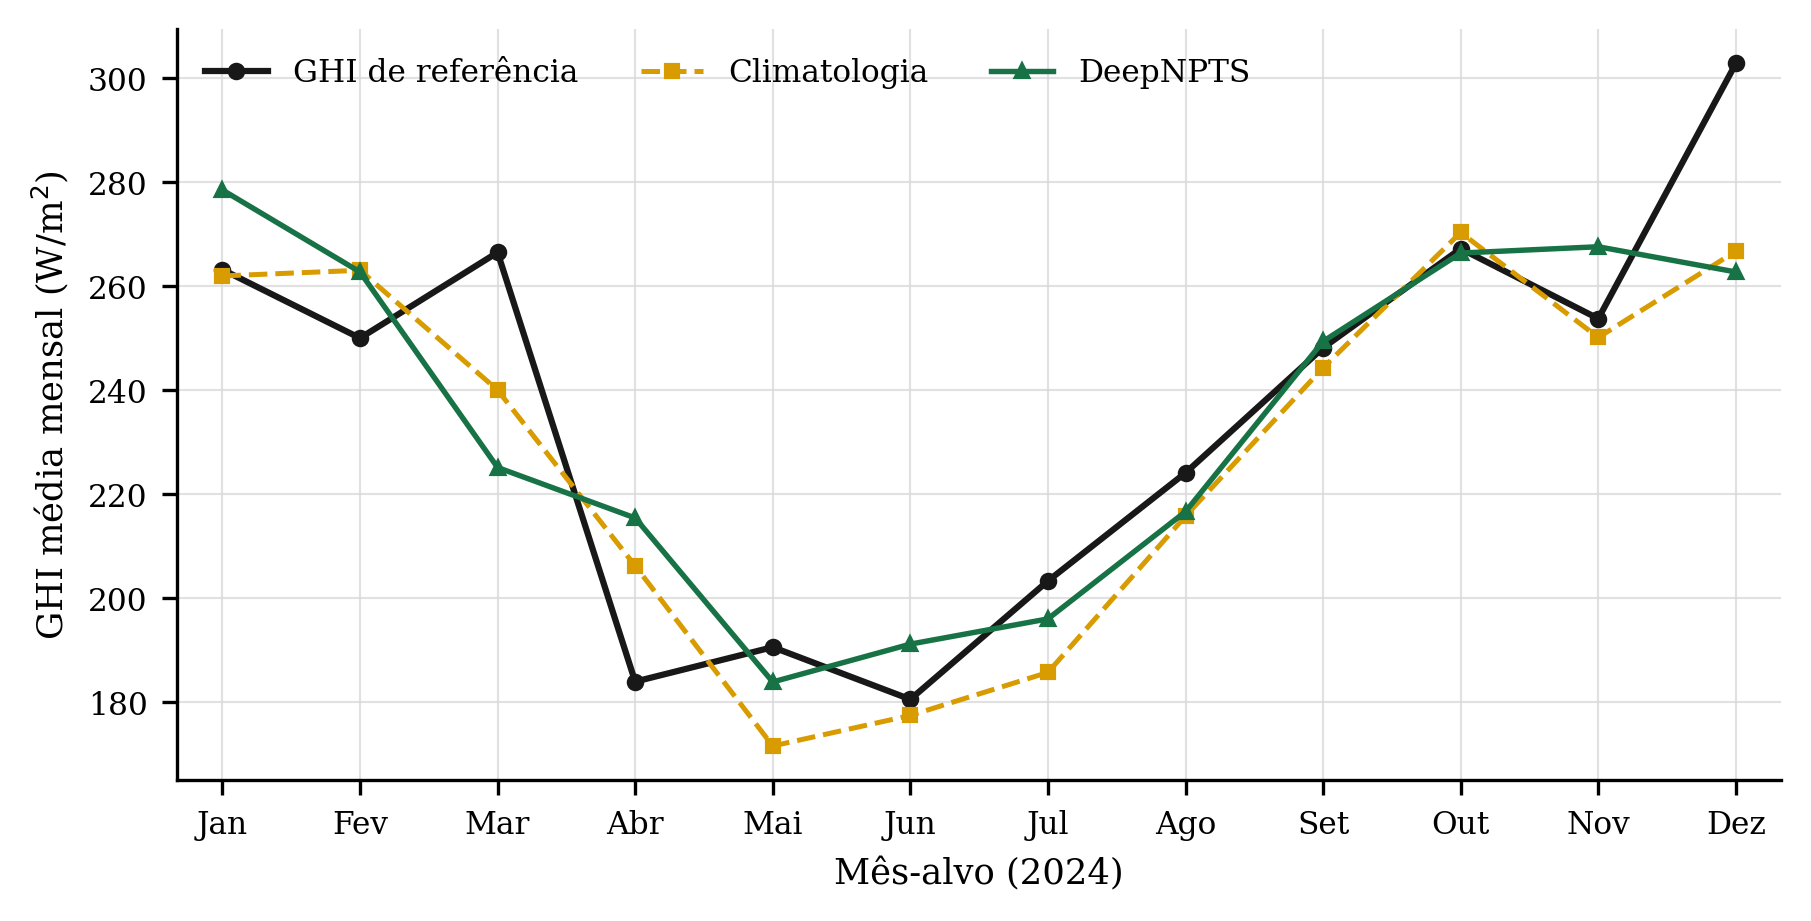
\includegraphics[width=\columnwidth]{previsao_mensal_byd_camacari.png}
\footnotesize (a) Referência e previsões pontuais.\par
\vspace{2pt}
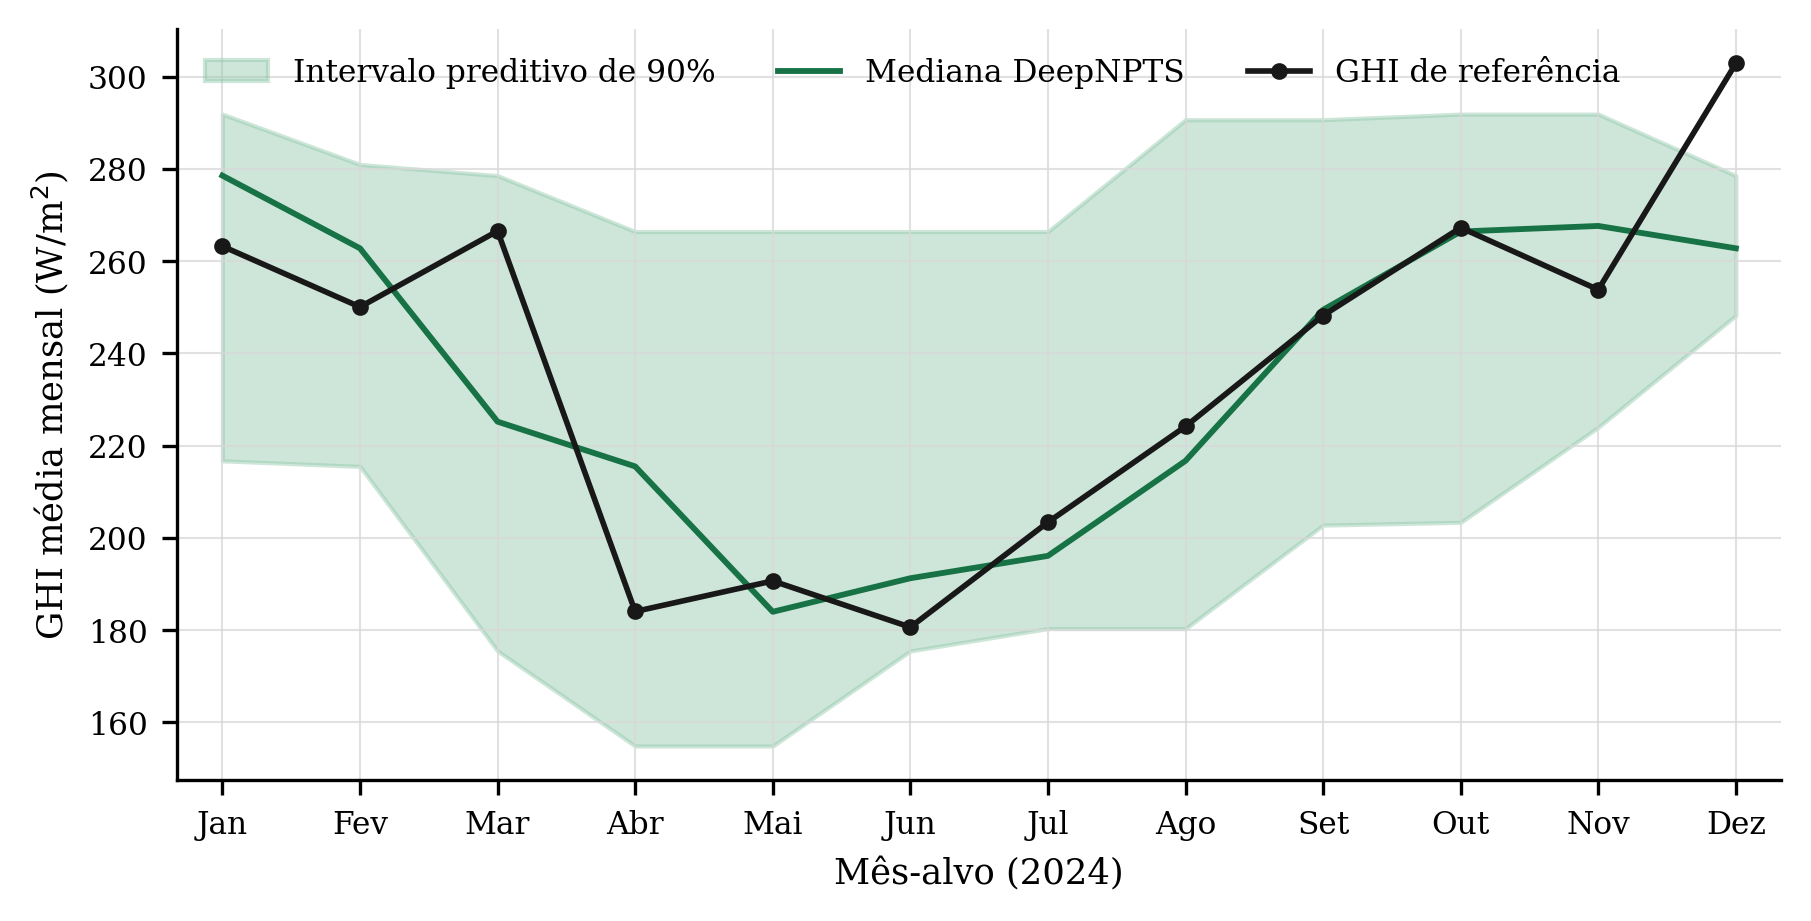
\includegraphics[width=\columnwidth]{intervalo_deepnpts_byd_camacari.png}
\footnotesize (b) Mediana e intervalo central de 90\%.
\caption{GHI de referência modelada da NSRDB e previsões para a BYD Camaçari
em 2024: (a) DeepNPTS e climatologia; (b) distribuição
preditiva do DeepNPTS.}
\label{fig:painel_byd}
\end{figure}

Na média entre localidades, o DeepNPTS apresentou CRPS de 15,90 W/m$^2$,
PICP$_{90}$ de 90,83\% e MPIW$_{90}$ de 145,56 W/m$^2$; para o DeepAR, os
valores foram 10,83 W/m$^2$, 61,67\% e 35,50 W/m$^2$. Assim, o DeepNPTS ficou
mais próximo da cobertura nominal, mas o DeepAR obteve menor CRPS; os
intervalos do DeepNPTS foram 4,10 vezes mais largos. As três métricas provêm
da mistura das amostras das cinco sementes.

\subsection{Limitações}

O histórico cobre seis anos, mas somente quatro ciclos fornecem alvos de
treinamento.

A janela de 2024 já foi examinada, e cinco sementes capturam somente parte da
variabilidade computacional.

As dez localidades foram
escolhidas pela presença das fábricas e não constituem amostra espacial
aleatória. Além disso, a transformação satura entradas fora dos extremos
pré-teste e a quantização discretiza os valores fornecidos aos modelos
aprendidos, enquanto as referências simples usam valores físicos exatos. A
NSRDB é uma referência modelada, e os dados horários brutos não foram
preservados. Os resultados não devem ser extrapolados para geração
fotovoltaica, dados industriais ou outras regiões sem nova validação.

\section{Conclusões}
\label{sec:conclusoes}

Este trabalho avaliou o DeepNPTS discreto na previsão mensal de GHI. Os modelos
aprendidos foram ajustados globalmente por semente e avaliados nas mesmas
origens retrospectivas.

No protocolo estudado, a climatologia obteve o menor macro-MAE,
12,07 W/m$^2$. O DeepNPTS alcançou 17,70 W/m$^2$, ficou em 9º lugar entre 10
métodos e superou apenas a persistência. Em relação ao DeepAR, o DeepNPTS teve
MAE pontual e CRPS maiores; sua cobertura ficou mais próxima de 90\%, mas seus
intervalos foram 4,10 vezes mais largos. Esses achados respondem à pergunta
experimental nesta janela, sem estabelecer superioridade universal.

Trabalhos futuros devem ampliar o histórico, reservar uma janela prospectiva e
avaliar outros horizontes, variáveis meteorológicas, saturação e quantização.

\balance
\begin{thebibliography}{99}

\bibitem{antonanzas2016}
J. Antonanzas et al., ``Review of photovoltaic power forecasting,''
\textit{Solar Energy}, vol. 136, pp. 78--111, 2016,
doi: 10.1016/j.solener.2016.06.069.

\bibitem{voyant2017}
C. Voyant et al., ``Machine learning methods for solar radiation forecasting:
A review,'' \textit{Renewable Energy}, vol. 105, pp. 569--582, 2017,
doi: 10.1016/j.renene.2016.12.095.

\bibitem{yang2018}
D. Yang et al., ``History and trends in solar irradiance and PV power
forecasting: A preliminary assessment and review using text mining,''
\textit{Solar Energy}, vol. 168, pp. 60--101, 2018,
doi: 10.1016/j.solener.2017.11.023.

\bibitem{duffie2013}
J. A. Duffie and W. A. Beckman, \textit{Solar Engineering of Thermal
Processes}, 4th ed. Hoboken, NJ, USA: Wiley, 2013.

\bibitem{sengupta2018}
M. Sengupta et al., ``The National Solar Radiation Data Base (NSRDB),''
\textit{Renewable and Sustainable Energy Reviews}, vol. 89, pp. 51--60, 2018,
doi: 10.1016/j.rser.2018.03.003.

\bibitem{voyant2022}
C. Voyant et al., ``Benchmarks for solar radiation time series forecasting,''
\textit{Renewable Energy}, vol. 191, pp. 747--762, 2022,
doi: 10.1016/j.renene.2022.04.065.

\bibitem{sobri2018}
S. Sobri, S. Koohi-Kamali, and N. A. Rahim, ``Solar photovoltaic generation
forecasting methods: A review,'' \textit{Energy Conversion and Management},
vol. 156, pp. 459--497, 2018, doi: 10.1016/j.enconman.2017.11.019.

\bibitem{chen2016}
T. Chen and C. Guestrin, ``XGBoost: A scalable tree boosting system,'' in
\textit{Proc. 22nd ACM SIGKDD Int. Conf. Knowledge Discovery and Data Mining},
2016, pp. 785--794, doi: 10.1145/2939672.2939785.

\bibitem{hornik1989}
K. Hornik, M. Stinchcombe, and H. White, ``Multilayer feedforward networks are
universal approximators,'' \textit{Neural Networks}, vol. 2, no. 5,
pp. 359--366, 1989, doi: 10.1016/0893-6080(89)90020-8.

\bibitem{elman1990}
J. L. Elman, ``Finding structure in time,'' \textit{Cognitive Science},
vol. 14, no. 2, pp. 179--211, 1990,
doi: 10.1207/s15516709cog1402\_1.

\bibitem{hochreiter1997}
S.~Hochreiter and J.~Schmidhuber, ``Long short-term memory,''
\textit{Neural Computation}, vol. 9, no. 8, pp. 1735--1780, 1997,
doi: 10.1162/neco.1997.9.8.1735.

\bibitem{chang2017}
S. Chang et al., ``Dilated recurrent neural networks,'' in
\textit{Advances in Neural Information Processing Systems}, vol. 30, 2017.

\bibitem{salinas2020}
D. Salinas, V. Flunkert, J. Gasthaus, and T. Januschowski, ``DeepAR:
Probabilistic forecasting with autoregressive recurrent networks,''
\textit{International Journal of Forecasting}, vol. 36, no. 3,
pp. 1181--1191, 2020, doi: 10.1016/j.ijforecast.2019.07.001.

\bibitem{rangapuram2023}
S. S. Rangapuram et al., ``Deep non-parametric time series forecaster,''
\textit{arXiv preprint arXiv:2312.14657}, 2023,
doi: 10.48550/arXiv.2312.14657.

\bibitem{alexandrov2020}
A. Alexandrov et al., ``GluonTS: Probabilistic and neural time series modeling
in Python,'' \textit{Journal of Machine Learning Research}, vol. 21, no. 116,
pp. 1--6, 2020.

\bibitem{nlr2026}
National Laboratory of the Rockies, ``GOES Aggregated PSM v4 Download API,''
2026. [Online]. Available:
\url{https://developer.nlr.gov/docs/solar/nsrdb/nsrdb-GOES-aggregated-v4-0-0-download/}.
Accessed: Jul. 19, 2026.

\bibitem{hyndman2006}
R. J. Hyndman and A. B. Koehler, ``Another look at measures of forecast
accuracy,'' \textit{International Journal of Forecasting}, vol. 22, no. 4,
pp. 679--688, 2006, doi: 10.1016/j.ijforecast.2006.03.001.

\bibitem{gneiting2007}
T. Gneiting and A. E. Raftery, ``Strictly proper scoring rules, prediction, and
estimation,'' \textit{Journal of the American Statistical Association},
vol. 102, no. 477, pp. 359--378, 2007,
doi: 10.1198/016214506000001437.

\end{thebibliography}

\end{document}
